\documentclass[letterpaper,12pt,oneside]{book}

\usepackage[utf8]{inputenc}
\usepackage[spanish,es-nodecimaldot,es-tabla]{babel}
\usepackage{graphicx}
\usepackage{multirow}
\usepackage{natbib}  % Usando paquete para citas
\usepackage{amsmath} % Notación
\usepackage{amssymb}
\usepackage{amsthm}  % Definiciones
\usepackage{longtable}
\usepackage{siunitx}
\usepackage{todonotes}   % insert [disable] to disable all notes
\usepackage[T1]{fontenc} % Required for accented characters
\usepackage{outlines}
\usepackage{url}
\usepackage{soul}  % Tachar caracteres
\usepackage{tipa} % Caracteres IPA
\usepackage{smartdiagram}
\usepackage{color, colortbl}

\definecolor{Yellow}{rgb}{1, 0.78, 0.26}

\newcommand{\note}[4][]{\todo[author=#2,color=#3,size=\scriptsize,fancyline,caption={},#1]{#4}} % default

%For comments in a bubble on the document margins:
\newcommand{\ximena}[2][]{\note[#1]{Ximena}{green!40}{#2}}
\newcommand{\vic}[2][]{\note[#1]{Vic}{orange!40}{#2}}
\newcommand{\diego}[2][]{\note[#1]{Diego}{blue!40}{#2}}

%For inline comments:
\newcommand{\Ximena}[2][]{\ximena[inline,#1]{#2}\noindent}
\newcommand{\Vic}[2][]{\vic[inline,#1]{#2}\noindent}
\newcommand{\Diego}[2][]{\diego[inline,#1]{#2}\noindent}

% For code formatting
\def\code#1{\texttt{#1}}

% Teoremas y ejemplos
\theoremstyle{definition}
\newtheorem{exmp}{Ejemplo}[section]
\newtheorem{definition}{Definición}

\graphicspath{{./img/}}

\begin{document}
\bibliographystyle{acl_natbib}  % Cargando estilo de bibliografia

\author{Diego Alberto Barriga Martínez}
\title{Etiquetador automático de la morfología del otomí usando predicción estructurada}
\maketitle
\tableofcontents

\chapter{Introducción}

% capítulo corto con el objetivo, hipótesis y tocar los temas del marco teorico de forma muy superficial. Se definen en el marco teorico

\section{Lengua otomí}

En esta sección se menciona los lugares donde se describe el idioma otomí de forma somera, se mencionan algunos lugares donde es hablado el otomí y características fundamentales de la lengua.

\subsection{Origen}

% Pie de pagina, no meter cosas tangenicales. Citar esta definicion
La palabra otomí es de origen náhuatl (singular: \textit{otomitl}, plural: \textit{otomí}). Por otra parte, los otomíes se nombran a sí mismos \textit{ñähñu}\footnote{Existen organizaciones indígenas, como el Consejo de la Nacionalidad Otomí, que escriben la auto-denominación como hñätho hñähñu y también ñätho ñähño. Sin embargo, esta auto denominación puede variar.}, que significa "los que hablan otomí".

Los grupos indígenas que hablan el idioma otomí se encuentran en diversas partes del territorio mexicano como: Estado de México, Querétaro, Hidalgo, Puebla y Veracruz \citep{barrientos2004otomies}. El otomí es una lengua indígena una gran variación dialectal que depende de su distribución geográfica.

En el Estado de México el pueblo \textit{ñähñu} está disperso por varios municipios tales como: Toluca, Lerma, Chapa de Mota, Aculco, Amanalco, Atizapán de Zaragoza, por mencionar algunos. En otros municipios como Naucalpan, Ecatepec, Nezahualcóyotl y Tlalnepantla se pueden encontrar hablantes por efectos de la migración. Según \citet{barrientos2004otomies} la población total de hablantes otomíes en el Estado de México supera los cien mil, sin embargo, datos actuales .

En concreto existen \textbf{nueve} variantes del otomí y cabe recalcar que dicha variación puede presentarse incluso dentro del mismo estado. Tan solo el Estado de México presenta tres variantes del otomí: El otomí de Tilapa, hablado en el municipio de Santiago Tianguistenco; el Otomí de Acazulco, del municipio de San Jerónimo Acazulco; y el Otomí de Toluca, de San Andrés Cuexcontitlán.

\section{Problemática}

El NLP es un área de la computación que permite reconocer, procesar e interpretar el lenguaje humano dentro de un sistema computacional. El objetivo de esta área es hacer que las computadoras realicen tareas que involucran el lenguaje humano. Algunas tareas generales consisten en permitir la comunicación humano-máquina, o simplemente hacer un exitoso procesamiento de texto o voz humanos \citep{jurafsky2008speech}. Ejemplos de aplicación actuales son los traductores automáticos, asistentes personales que reconocen voz, motores de búsquedas en Internet, análisis de sentimientos en textos,  síntesis de voz, etiquetado de textos y muchas más aplicaciones.

% Voy de lo mas general a lo particular
Una de las tareas más populares de NLP es el etiquetado automático de textos. Este etiquetado puede realizarse a diferentes niveles lingüísticos, por ejemplo, morfosintáctico (\textit{Part Of Speech tagging, POS}), sintáctico (\textit{parsing}), morfológico, etc.  El nivel morfológico tiene que ver con la estructura interna de las palabras \citep{haspelmath2013understanding}; en particular, existe un tipo de etiquetado, de gran importancia para el análisis lingüístico, llamado glosado que asigna etiquetas a las unidades que conforman a una palabra. 

% Hablando de ML
Para lograr lo anterior, los enfoques actuales aplican técnicas de ML. El ML es un subcampo de la Inteligencia Artificial (IA), que constituye un enfoque de resolución de problemas caracterizado por estimar una solución a partir de la experiencia \citep{mitchell1997machine}.  La experiencia se refiere a datos etiquetados (ejemplos) que permiten inferir un modelo estadístico de aprendizaje. Entre los métodos de ML ampliamente utilizados se pueden mencionar las Support Vector Machines (SVMs), árboles de decisión, o bien los modelos gráficos, como las redes neuronales o los métodos generativos, solo por mencionar algunos. Para las tareas de etiquetado en NLP generalmente se utilizan modelos gráficos supervisados, por ejemplo, modelos ocultos de Markov (\textit{Hidden Markov Models, HMM}).

% Introduccion de la problematica
No obstante, el lenguaje natural es complejo y dinámico, ya que tiene fenómenos que hacen que las tareas de reconocimiento, generación y procesamiento se vuelvan difíciles para las computadoras. Adicionalmente, existen escenarios donde estos métodos no son efectivos como es el caso de las lenguas de bajos recursos, que son lenguas que tienen pocos recursos digitales con los que trabajar. Por ejemplo, si se tienen pocos datos iniciales para el entrenamiento del modelo de aprendizaje las predicciones serán poco precisas o equivocadas. Los bajos recursos son un escenario común en México donde, a pesar de que existe una rica diversidad lingüística, gran parte de las lenguas originarias no poseen contenido web ni publicaciones digitales y por tanto carecen también de tecnologías del lenguaje.  El escenario mencionado anteriormente supone un reto para los métodos de aprendizaje convencionales, que requieren de grandes cantidades de datos de entrenamiento para funcionar correctamente. Por lo tanto, es un importante reto de investigación desarrollar aproximaciones que funcionen con lenguas de escasos recursos. En particular, en este trabajo nos enfocamos en el glosado automático del otomí, una lengua con gran riqueza morfológica y con escasez de recursos digitales.

El glosado puede ser un primer paso para el desarrollo de más tecnologías del lenguaje; no solo para el otomí, que presenta un grado de extinción acelerada (Comisión Nacional para el Desarrollo Indígena)\footnote{https://www.gob.mx/inpi}, sino para las 68 agrupaciones lingüísticas que se hablan en México.

\section{Objetivo}

Diseñar e implementar un etiquetador morfológico para el otomí basado en técnicas de Procesamiento del Lenguaje Natural (\textit{Natural Language Processing, NLP}) con Aprendizaje de Máquina (\textit{Machine Learning, ML}). En particular, se hará énfasis en métodos de aprendizaje estructurado débilmente supervisados. Específicamente, se aplicará \textit{Conditional Random Fields (CRF)} para etiquetado morfológico (glosado) del otomí, una lengua de bajos recursos.

\section{Hipótesis}

Se espera obtener un modelo que produzca glosa para el otomí, generada automáticamente, con base en el entrenamiento con pocos ejemplos previamente etiquetados. Al obtener una buena exactitud en la predicción automática de glosa se apoyaría a los anotadores humanos a reducir trabajo repetitivo y exhaustivo. Además, se espera obtener avances de una metodología adaptable a un mayor número de lenguas mexicanas. Sería deseable que esta metodología experimental pueda ser replícale en otras lenguas habladas en México.

\chapter{Avances en etiquetadores automáticos}

% Mencionar los bajos recursos

\section{Marco teórico}\label{sec:marco}

% Se tiene que explicar los conceptos de low resouces 

% Etiquetadores a diferentes niveles lingüísticos
% Etiquetadores a nivel morfológico
% modelos gráficos
% Que es un etiquetador
% Bio Labels
% Que es la morfología 
% que es la glosa
% Low resources
% Algoritmo L&BFGS
    % L1/L2

% NLP
\subsection{Natural Language Processing (NLP)}
% Introduccion

\subsection{Etiquetadores}

% Machine learning
\subsection{Machine Learning (ML)}

\subsection{Modelos gráficos}

% Los límites de los modelos gráficos para bajos recursos

% Cierre de los modelos gráficos y comenzar a hablar de CRF
% No perder de vista que los CRFs son modelos gráficos pero con ventajas

\subsubsection{Los límites de los modelos gráficos en para bajos recursos}

En este capítulo se explicará qué ventajas tienen los \emph{Conditional Random Fields (CRF)} sobre otros modelos de aprendizaje, se mencionan formalmente los elementos fundamentales que describen los \emph{CRF's}.

En lingüística computacional una tarea de interés es el procesamiento estadístico del lenguaje natural, en particular, el etiquetado y segmentación de secuencias de datos. En ese sentido, es habitual la utilización de \textbf{modelos generativos}, cómo los \textit{Hidden Markov Models (HMMs)}, o \textbf{modelos condicionales}, como los \textit{Maximum Entropy Markov Models (MEMMs)}.

Por una parte, los modelos generativos intentan modelar una probabilidad conjunta $P(x,y)$ sobre observaciones y etiquetas. Para definir esta probabilidad conjunta se necesita enumerar todas las observaciones posibles. Las limitantes de este enfoque son de diversas índoles como las grandes dimensionalidades en el vector de entrada $X$, la dificultad de representar múltiples características que interactúan unas con otras y dependencias complejas que hacen la construcción de la distribución de probabilidad un problema intratable con un enfoque computacional.

Por otro lado, una solución a las limitantes de los modelos generativos es un modelo condicional. Estos modelos no son tan estrictos como los primeros al momento de asumir independencias en las observaciones. Los modelos condicionales especifican la probabilidad de posibles etiquetas dada una secuencia de observación.

Consecuencia de lo anterior, no se gasta esfuerzo en modelar las observaciones, dado que en al momento de realizar pruebas estas observaciones son fijas. Segundo, la probabilidad condicional puede depender de características arbitrarias y no dependientes de la secuencia de observación sin forzar al modelo a tomar en cuenta la distribución de estas características, permitiendo que el modelo sea tratable \citep{lafferty2001conditional}.

Un ejemplo de estas ventajas con los \textit{MEMMs} que son modelos secuenciales de probabilidad condicional. Sin embargo, estos modelos y otros que son no generativos, de estados finitos y que son clasificadores basados en el estado siguiente comparten una debilidad llamada \emph{label bias problem}. \citet{lafferty2001conditional} define que existe el \emph{label bias problem} cuando "las transiciones que dejan un estado compiten solo entre sí, en lugar de entre todas las demás transiciones en el modelo".

Dado que las transiciones son las probabilidades condicionales de los siguientes posibles estados una observación puede afectar cuál será el estado siguiente sin tomar en cuenta que tan adecuado será este. Por tanto, se tendrá un sesgo en los estados con menos transiciones de salida.

\subsection{Conditional Random Fields}

Como menciona \citet{sutton2012introduction} modelar las dependencias entre las entrada puede conducir a modelos intratables, pero ignorar estas dependencias puede reducir el rendimiento.

Dado el que problema abordado en este trabajo, dónde se requiere del etiquetado de secuencias y es en contexto de bajos recursos lingüísticos, se hace necesario utilizar un enfoque más conveniente.

Los \textit{Conditional Random Fields (CRFs)} son un framework para la creación de modelos probabilístico utilizado en técnicas de aprendizaje estructurado. Tienen las ventajas de los \textit{MEMMs} y, en principio, solucionan el \emph{label bias problem}. El framework tiene un solo modelo exponencial para la probabilidad conjunta de todas las secuencias de las etiquetas de salida dada la secuencia de observación. En contraste los \emph{MEMMs} usan modelos exponenciales para cada probabilidad condicional de los estados siguientes dado el estado actual.

Formalmente \citet{lafferty2001conditional} definen los \textit{CRFs} como a continuacion se enuncia:

\begin{definition}
	Sea $G = (V,E)$ una gráfica tal que $\mathbf{Y} = (\mathbf{Y}_{v})_{v \in V}$, entonces esa $\mathbf{Y}$ es indexada por los vertices de $G$. Entonces $(\mathbf{X}, \mathbf{Y})$ es un \textsf{conditional random field} en caso de que las variables aleatorias $\mathbf{Y}$ se condicionen por $\mathbf{X}$, la variable aleatoria $\mathbf{Y}_{v}$ cumple la \textit{propiedad de Markov} con respecto a la gráfica: $p(\mathbf{Y}_{v}|\mathbf{X},\mathbf{Y}_{w},w \ne v) = p(\mathbf{Y}_{v}|\mathbf{X},\mathbf{Y}_{w},w \sim v)$, dónde $w \sim v$ significa que $w$ y $v$ son vecinos en $G$.
\end{definition}

En esta tesis, para el modelado de secuencias, se utiliza la forma más sencilla de la gráfica $G$ dónde es una cadena simple o línea. Esto quiere decir que $G = (V = \{1,2,...m\}, E = \{(i,i+1)\})$. A este tipo de \textit{CRFs} se les conoce como \textit{linear-chain CRFs}. Como menciona \citet{lafferty2001conditional} "si la gráfica $G = (V,E)$ de $\mathbf{Y}$ es un árbol (del cual una cadena es el ejemplo más sencillo), los \textit{cliques} son los límites y vertices. Entonces, por el teorema de los \textit{random fields} \citep{hammersley1971markov}, la distribución conjunta sobre las etiquetas de secuencias $\mathbf{Y}$ y $\mathbf{X}$ tiene la forma:

% TODO: Poner tag
% TODO: Explicar esta ecuacion sobre que es son las lambdas, porque hay dos sumandos, porque el símbolo de proporcionalidad, 
\begin{equation}
    p{_{\theta}}(y|x) \propto \exp \bigg( \sum\limits_{e \in \mathbf{E},k} \lambda_{k}f_{k}(e,\mathbf{y}|_{e},\mathbf{x}) + \sum\limits_{v \in \mathbf{V},k}\mu_{k}g_{k}(v,\mathbf{y}|_{v},\mathbf{x}) \bigg)
\end{equation}

% TODO: Mencionar la ecucacion
% TODO: Descripcion de la estimacion de parametros y característica de la función de perdida

De la ecuación  se destacan $f_{k}$ y $g_{k}$ que representan las \textit{feature functions}. Estas están definidas y son fijas. Las \textit{feature functions} de está tesis serán descritas más adelante. 


\section{Estado del arte}

Los \textit{CRFs} han sido utilizados para la clasificación de regiones en una imagen, estimar el puntaje en un juego de Go, segmentar genes en una hebra de ADN y análisis sintáctico de lenguaje natural en un texto por mencionar algunas \citep{sutton2012introduction}.


\subsection{Trabajos sobre bajos recursos}
% Hablar del trabajo para Lezgi
Con base en el trabajo previo de \citep{moeller2018automatic} donde se utilizan técnicas de NLP y ML para tratar para el idioma Lezgi se plantea como hipótesis que dado el tamaño del corpus y la glosa que contiene 
se obtendrá texto correctamente glosado con una precisión de al menos 80\%.

\Diego{Descripción de la estimación de parámetros y característica de la función de perdida}
% Papers que hablen del tema de etiquetado automático 2010 para acá

% Redes neuronales,
% Mención de trabajo y papers actuales hacen algo similar

%%%%%%%%%%%%%%%%%%%%%%%%%%%%%%%%%%%%%%%%%%%%%%%%%%%%%
% Metoodologia 
%%%%%%%%%%%%%%%%%%%%%%%%%%%%%%%%%%%%%%%%%%%%%%%%%%%%%

\chapter{Etiquetador morfológico para el otomí (Metodología)} \label{chap:metodology}

El objetivo de este capítulo es la presentación de la metodología utilizada en esta tesis. La metodología está constituida por un corpus etiquetado, del cual se incluye una descripción detallada, y la arquitectura para la generación de glosa para el idioma otomí. La arquitectura incluye, entre otras cosas, la codificación y preprocesamiento del corpus, el diseño e implementación del los \textit{CRFs} y la determinación de las \textit{feature functions}.

El punto principal de la metodología fue la implementación de los \textit{CRFs} que mostraron claras ventajas sobre otros métodos de aprendizaje basados en gráficas. Elegimos este \textit{framework} ya que se presenta como una opción para el contexto de los bajos recursos digitales que presenta el otomí, como se describirá más adelante. En ese sentido, la implementación de los \textit{CRFs} fue utilizada para predecir secuencias de etiquetas, con el enfoque del aprendizaje estructurado, que describen las unidades morfológicas dentro de una palabra de una variante del otomí. 

% Particularidades del corpus (Análisis cualitativo y cuantitativo)
\section{Corpus: otomí de Toluca}

% Tipo de otomi y características de la variante
La clasificación lingüística introduce al otomí dentro de las lenguas otomianas, las cuales a su vez pertenecen a la rama otopame de la familia otomangue \citep{barrientos2004otomies}. Cada variante muestra particularidades fonológicas, morfológicas, sintácticas y léxicas. En el tratamiento de textos por medio de técnicas de \textit{NLP} se requiere que estos textos estén normalizados y homogéneos. Dicha normalización propicia la obtención del mejor desempeño posible en los diversos métodos de aprendizaje automático. Más adelante se describirá el proceso de preprocesamiento aplicado al corpus que tuvo el propósito de adecuar el corpus a la arquitectura y normalizar el texto.

% Otomi en general, Familia y rama
Esta  tesis utilizó un corpus en otomí que, además, cumple la característica de estar glosado. Se trabajó con la variante del otomí de Toluca de la región de San Andrés Cuexcontitlan.

% De donde vienen los textos, quien lo glosa y quien lo recolecta
Se recogió un corpus basado en el trabajo de \citet{lastra1992otomi} titulado \emph{El otomí de Toluca} y que a su vez fue etiquetado y glosado manualmente por el lingüista Víctor Germán Mijangos de la Cruz\footnote{TODO: Liga del repo}. Este corpus es un subconjunto del corpus paralelo español-otomi que se encuentra en la plataforma web Tsunkua\footnote{https://tsunkua.elotl.mx/}.

% Tokens y tipos de Palabras

% Numero de etiquetas diferentes
\begin{table}
	\centering
	\begin{tabular}{c | c}
		\textbf{Categoría} & \textbf{Cuenta} \\ \hline
		Tokens (POS) & 8578\\
		Tipos (POS) & 44\\
		Tokens (Glosa) & 14477\\
		Tipos (Glosa) & 112\\
		\textbf{Total de oraciones etiquetadas} & 1786 \\ 
	\end{tabular}
	\caption{Tamaño del corpus}
	\label{table:corpus_length:1}
\end{table}

Además, se agregaron 81 lineas de casos poco usuales que son fenómenos poco frecuentes y, por tanto, particularmente difíciles de predecir. El subconjunto del corpus utilizado en la sección experimental está descrito en la tabla \ref{table:corpus_length:1}, donde se encuentra el tamaño de las etiquetas POS y el tamaño de la glosa y en la tabla \ref{table:corpus_text:1}, donde se puede ver los tipos de textos presentes en el corpus.

Los textos que componen el corpus fueron construidos a partir de las aportaciones de diez hablantes distintos de entre diez y setenta y tres años, de los cuales, siete son de sexo femenino y tres masculino \citep{lastra1992otomi}.

\begin{table}
	\centering
	\begin{tabular}{ c | c }
		\textbf{Textos} & \textbf{Número} \\ \hline
		Narrativos & 32 \\
		Dialogados & 4  \\
		\textbf{Total de textos}  & 36 \\
	\end{tabular}
	\caption{Textos del corpus}
	\label{table:corpus_text:1}
\end{table}

% Citar el estándar de etiquetas https://www.eva.mpg.de/lingua/pdf/Glossing&Rules.pdf
Los tipos de etiquetas \textit{POS} presentes en el corpus se pueden observar en la tabla \ref{table:pos_types}. Dentro del corpus se encontrón glosas que no corresponden a etiquetas \textit{POS}, sino que describen la semántica (traducciones) de las palabras. Como por ejemplo: en el fragmento en otomí \textsf{"...ná ra sapahtá pe lo prinsipal..."} ("...empezado un Zapata, pero lo principa...") \textsf{sapahtá} tendría como glosa la palabra \textsf{zapata} que es su traducción. Esta forma de presentar las etiquetas \textit{POS} es común en el uso lingüístico y no vale la pena presentarla en la tabla \ref{table:pos_types} pues son descriptivos por sí mismos. 

\begin{table}
	\centering
	\begin{tabular}{| c | c | c | c | c |}
		\hline
		v & obl & det & cnj & dem \\ 
		unkwn & n & neg & p.loc & prt \\
		conj.adv & dim & gen & cond & it \\
	    lim & aff & loc & dec & conj  \\
	    cord & san & cnj.adv & regular/v & adv \\
	    adj & & & & \\
	    \hline
	\end{tabular}
	\caption{Tipos de etiquetas \textit{POS}} 
	\label{table:pos_types}
\end{table}

Por otra parte, presentamos una descripción de las etiquetas \textit{POS} en la tabla \ref{table:pos_descr} dónde se muestra el significado de cada una. Por último, la distribución de las etiquetas \textit{POS}, se encuentra en la figura \ref{fig:pos_distrib}. En esta figura se muestra una carga importante hacia unas pocas etiquetas \textit{POS}. Esta característica es considerara por el modelo de aprendizaje estructurado que utilizamos y puede suponer un problema importante en métodos de aprendizaje convencionales.

\begin{table}
    \centering
    \begin{tabular}{| c  c | c  c |} \hline
		\textbf{Etiqueta} & \textbf{Significado} & \textbf{Etiqueta} & \textbf{Significado} \\ \hline
		v & verbo & obl & oblicuo \\
		det & determinante & cnj & conjunción \\
		dem & demostrativo & unkwn & desconocido\\ 
		n & sustantivo & neg & negativo \\
		p.loc & partícula locativoa & prt & partícula \\
		conj.adv & conjunción adversativa & dim & diminutivo \\
		gen & genitivo & cond & condicional\\
		it & iterativo & lim & limitativo \\ 
		aff & afirmativo & loc & locativo \\
		dec & decimal & conj & conjunción \\
	    cord & coordinación & cnj.adv & conjunción adversativa \\
	    regular/v & verbo regular & & \\
	    \hline
	\end{tabular}
	\caption{Descripción de etiquetas \textit{POS}}
	\label{table:pos_descr}
\end{table}


\begin{figure}
	\centering
	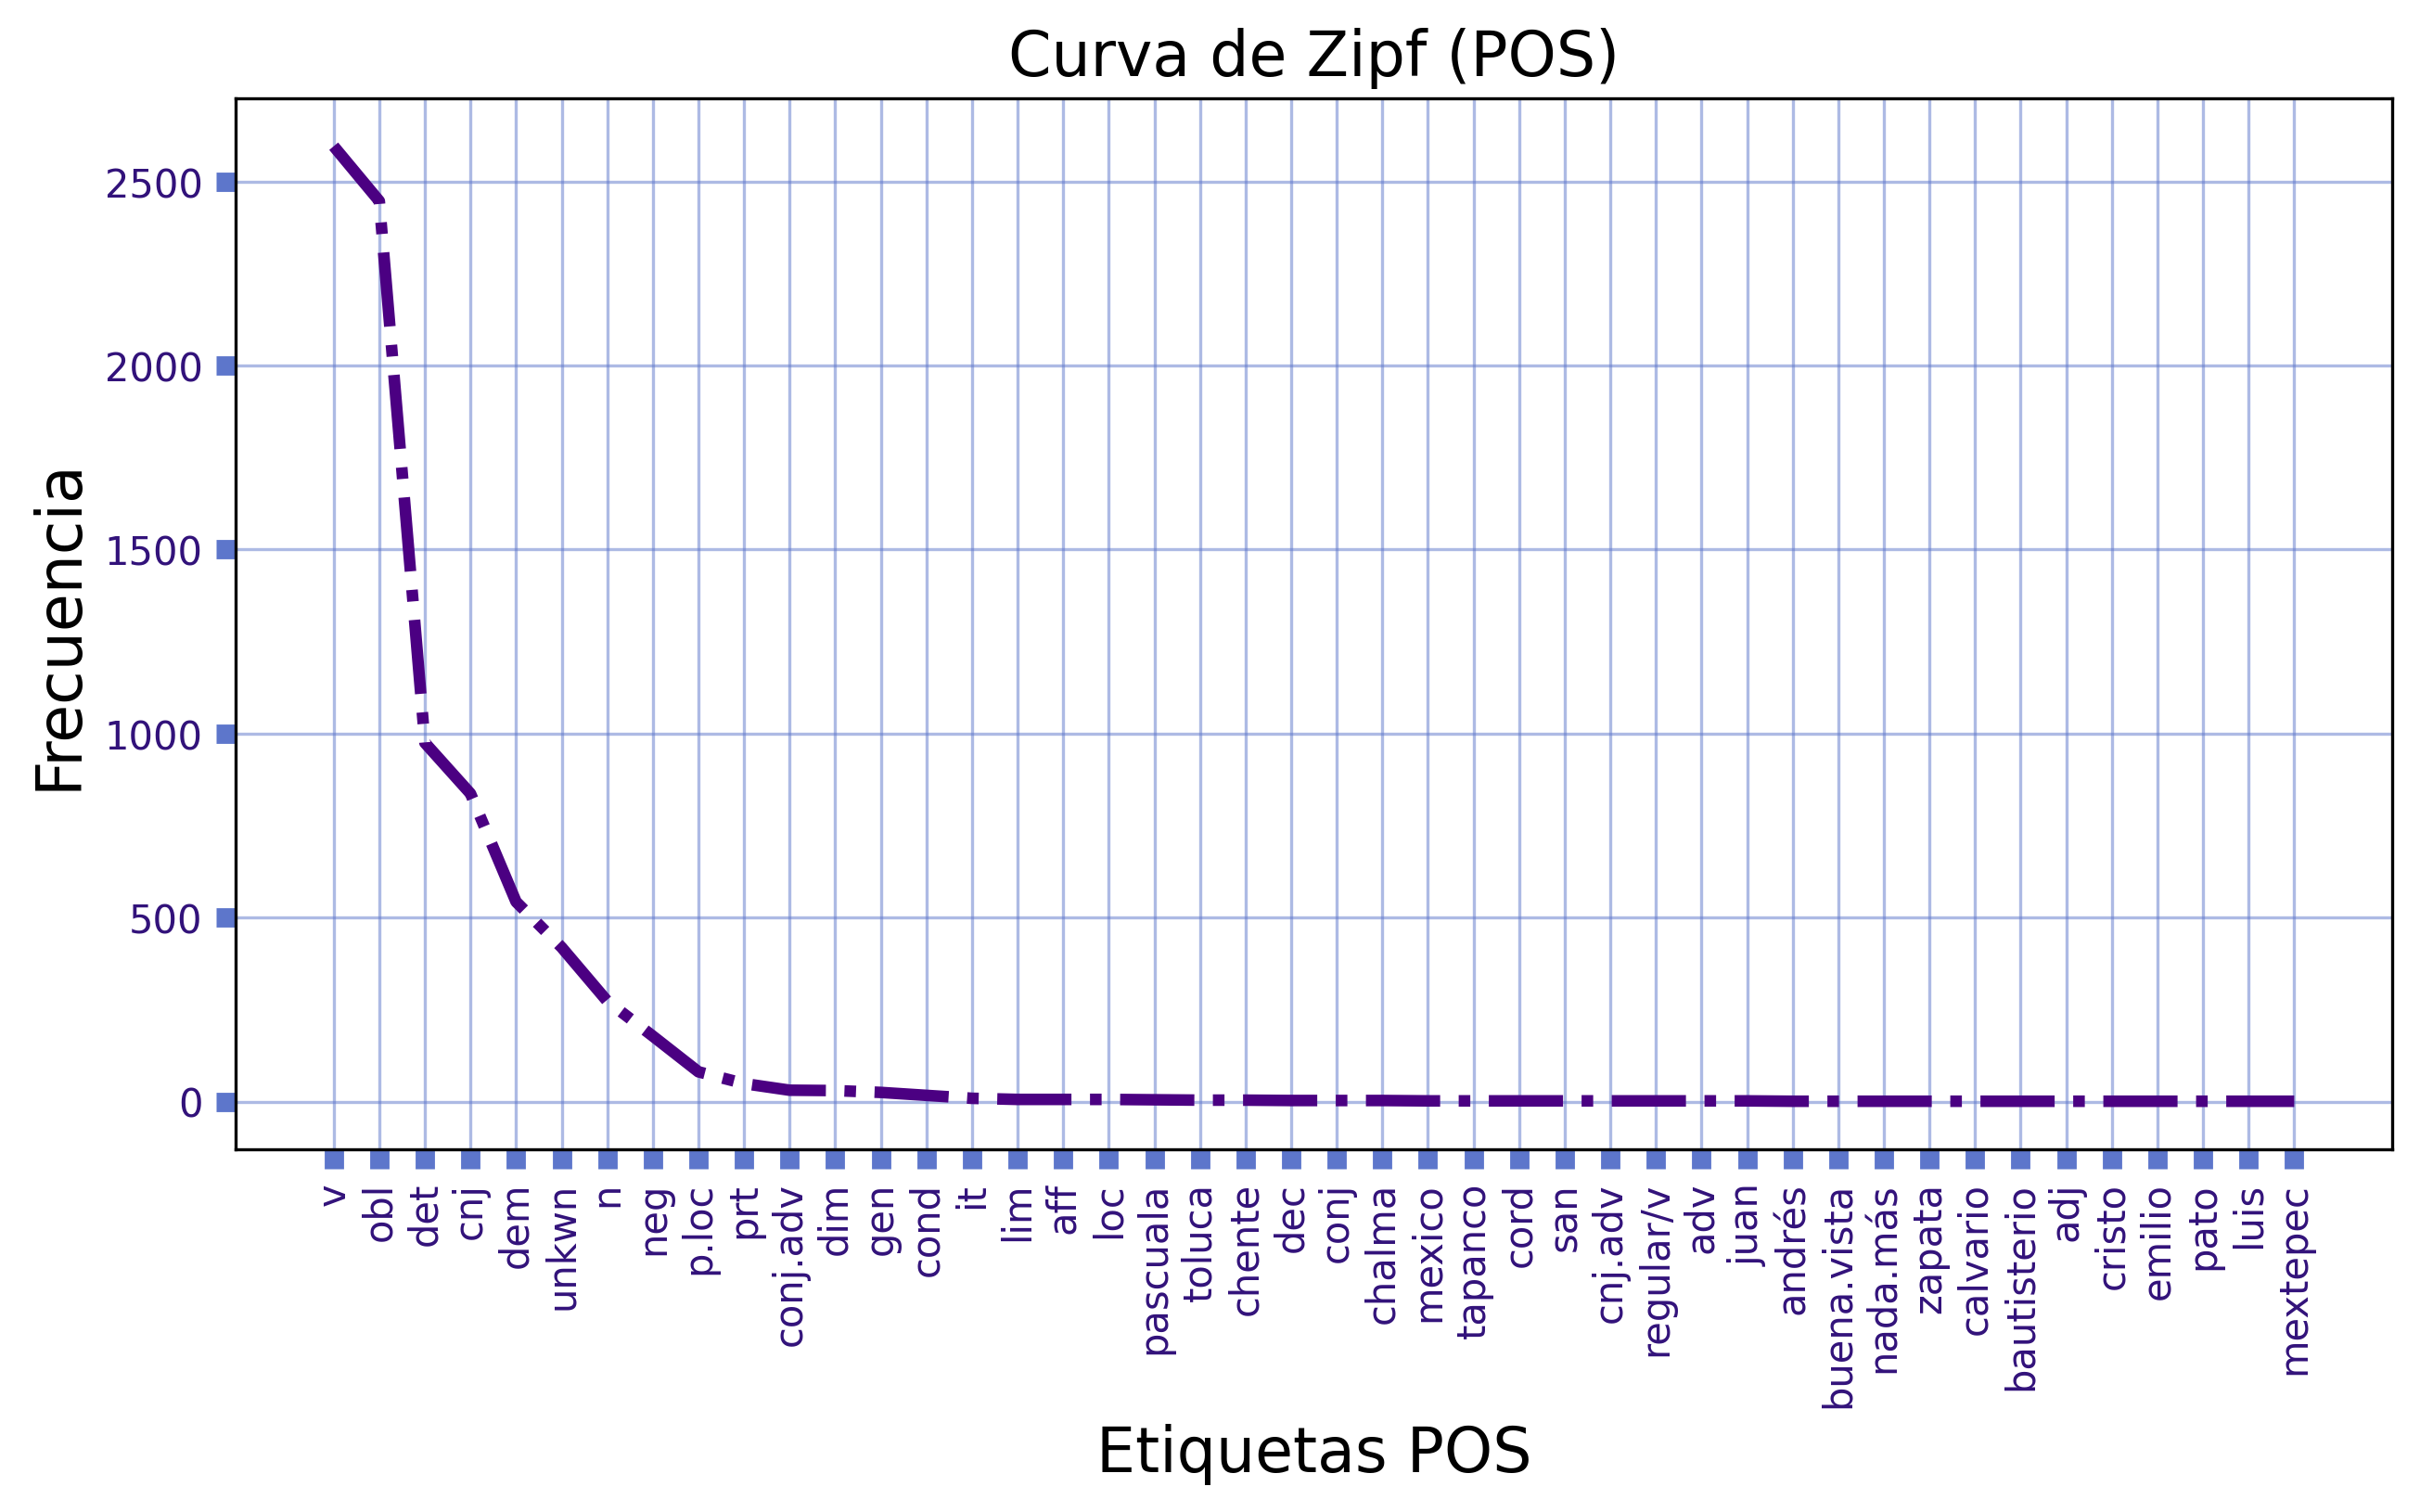
\includegraphics[width=\textwidth]{zipf_pos}
	\caption{Distribución de etiquetas POS}%\Vic{En escala logaritmica}
	\label{fig:pos_distrib}
\end{figure}

Para las etiquetas de Glosa nos basamos en las reglas de \citet{comrie2008leipzig} desarrolladas por el departamento de lingüística del Instituto Max Planck y el Departamento de lingüística de la Universidad de Leipzig. El estándar consiste en diez reglas para la sintaxis y la semántica de glosas interlineales. y un apéndice con un lexicón propuesto de etiquetas de categorías abreviadas \citep{comrie2008leipzig}. Si bien las reglas cubren parte de las necesidades lingüísticas en el glosado de textos, también, son flexibles y se pueden agregar o modificar las convenciones dependiendo de las necesidades.

Los tipos de etiquetas de glosa presentes en el corpus se encuentran en la tabla \ref{table:gloss_types}. En algunos casos aparecen números al inicio de etiquetas que significan las personas gramaticales. Existen combinaciones de varias etiquetas que son separadas por puntos. Por ejemplo, \textsf{pl.exc} es una combinación de las etiquetas ''plural'' y ''exclusivo''.

\begin{table}
	\centering
	\begin{tabular}{| c | c | c | c | c |}\hline
		 stem & det & 3.cpl & psd & lim \\
         prag & 3.icp & lig & det.pl & 1.icp \\
         3.pot & ctrf & 1.pot & pl.exc & 1.cpl \\
         dem & 1.pss & dim & pl & 1.obj \\
         ila & 2.icp & 1.prf & 3.cnt & 3.obj \\
         loc & mod & 1.cnt & 3.pls & prt \\
         it & dual.exc & 3.prf & 3.icp.irr & 3.pss \\
         2.pss & 1.enf & med & dual & p.loc \\
         2.cnt & 2 & 3.imp & int & neg \\
         1.icp.irr & 1.cpl.irr & 2.obj & aum & 1.pls \\
         2.cpl & 2.prf & gen & com & 2.pot\\
         adj & cond  & 3.cpl.irr & 1.sg & encl \\
         3.sg & 3.pss.pl & spt & 1.irr & 2.enf \\
         conj.adv & caus & con & chico & eh \\
         comp & prf & dist mov & 3.irr & det.dem\\
         dcl & nom & 2.icp.irr & & \\
		\hline
	\end{tabular}
	\caption{Glosa}
	\label{table:gloss_types}
\end{table}


El significado para cada etiqueta de glosa se muestra en la tabla \ref{table:gloss_desc}. En esta tabla se omitieron las variaciones de etiquetas con personas gramaticales para compactarla. Además, la distribución de las etiquetas presentes en el corpus se muestran en la figura \ref{fig:gloss_distrib}. Igual que en la figura \ref{fig:pos_distrib} se observa una carga pronunciada en la distribución hacia pocas etiquetas como \textsf{stem}. Este fenómeno es propiciado, en parte, a que son escasos los textos digitales disponibles para el idioma otomí.

\begin{table}
	\centering
	\begin{tabular}{ c  c | c  c }
		\textbf{Glosa} & \textbf{Significado} & \textbf{Glosa} & \textbf{Significado}\\\hline
		stem & base & ctrf & contrafactual \\
        cpl & completivo & dem & demostrativo \\
        icp & incompletivo & dim & diminutivo \\
        pot & potencial & ila & ilativo \\
        ctn & continuativo & mod & modo \\
        prf & perfecto & loc & locativo \\
        pls & pluscuamperfecto & prt & partícula \\
        irr & irrealis & it & iterativo \\
        imp & imperativo & enf & enfático \\
        psd & pasado & neg & negativo \\
        pl & plural & int & interrogativo \\
        sg & singular & aum & aumentativo \\
        ex & exclusivo & gen & genitivo \\
        pss & posesivo & com & comitativo \\
        obj & objeto & adj & adjetivo \\
        med & voz media & encl & enclítico \\
        dual & número dual & enf & enfático \\
        det & determinante & caus & causativo \\
        lim & limitativo & comp & comparativo \\
        lig & ligadura & dcl & declarativo \\
        prag & partícula pragmática & \\ \hline
	\end{tabular}
	\caption{Descripción de Glosa}
	\label{table:gloss_desc}
\end{table}
	

\begin{figure}
	\centering
	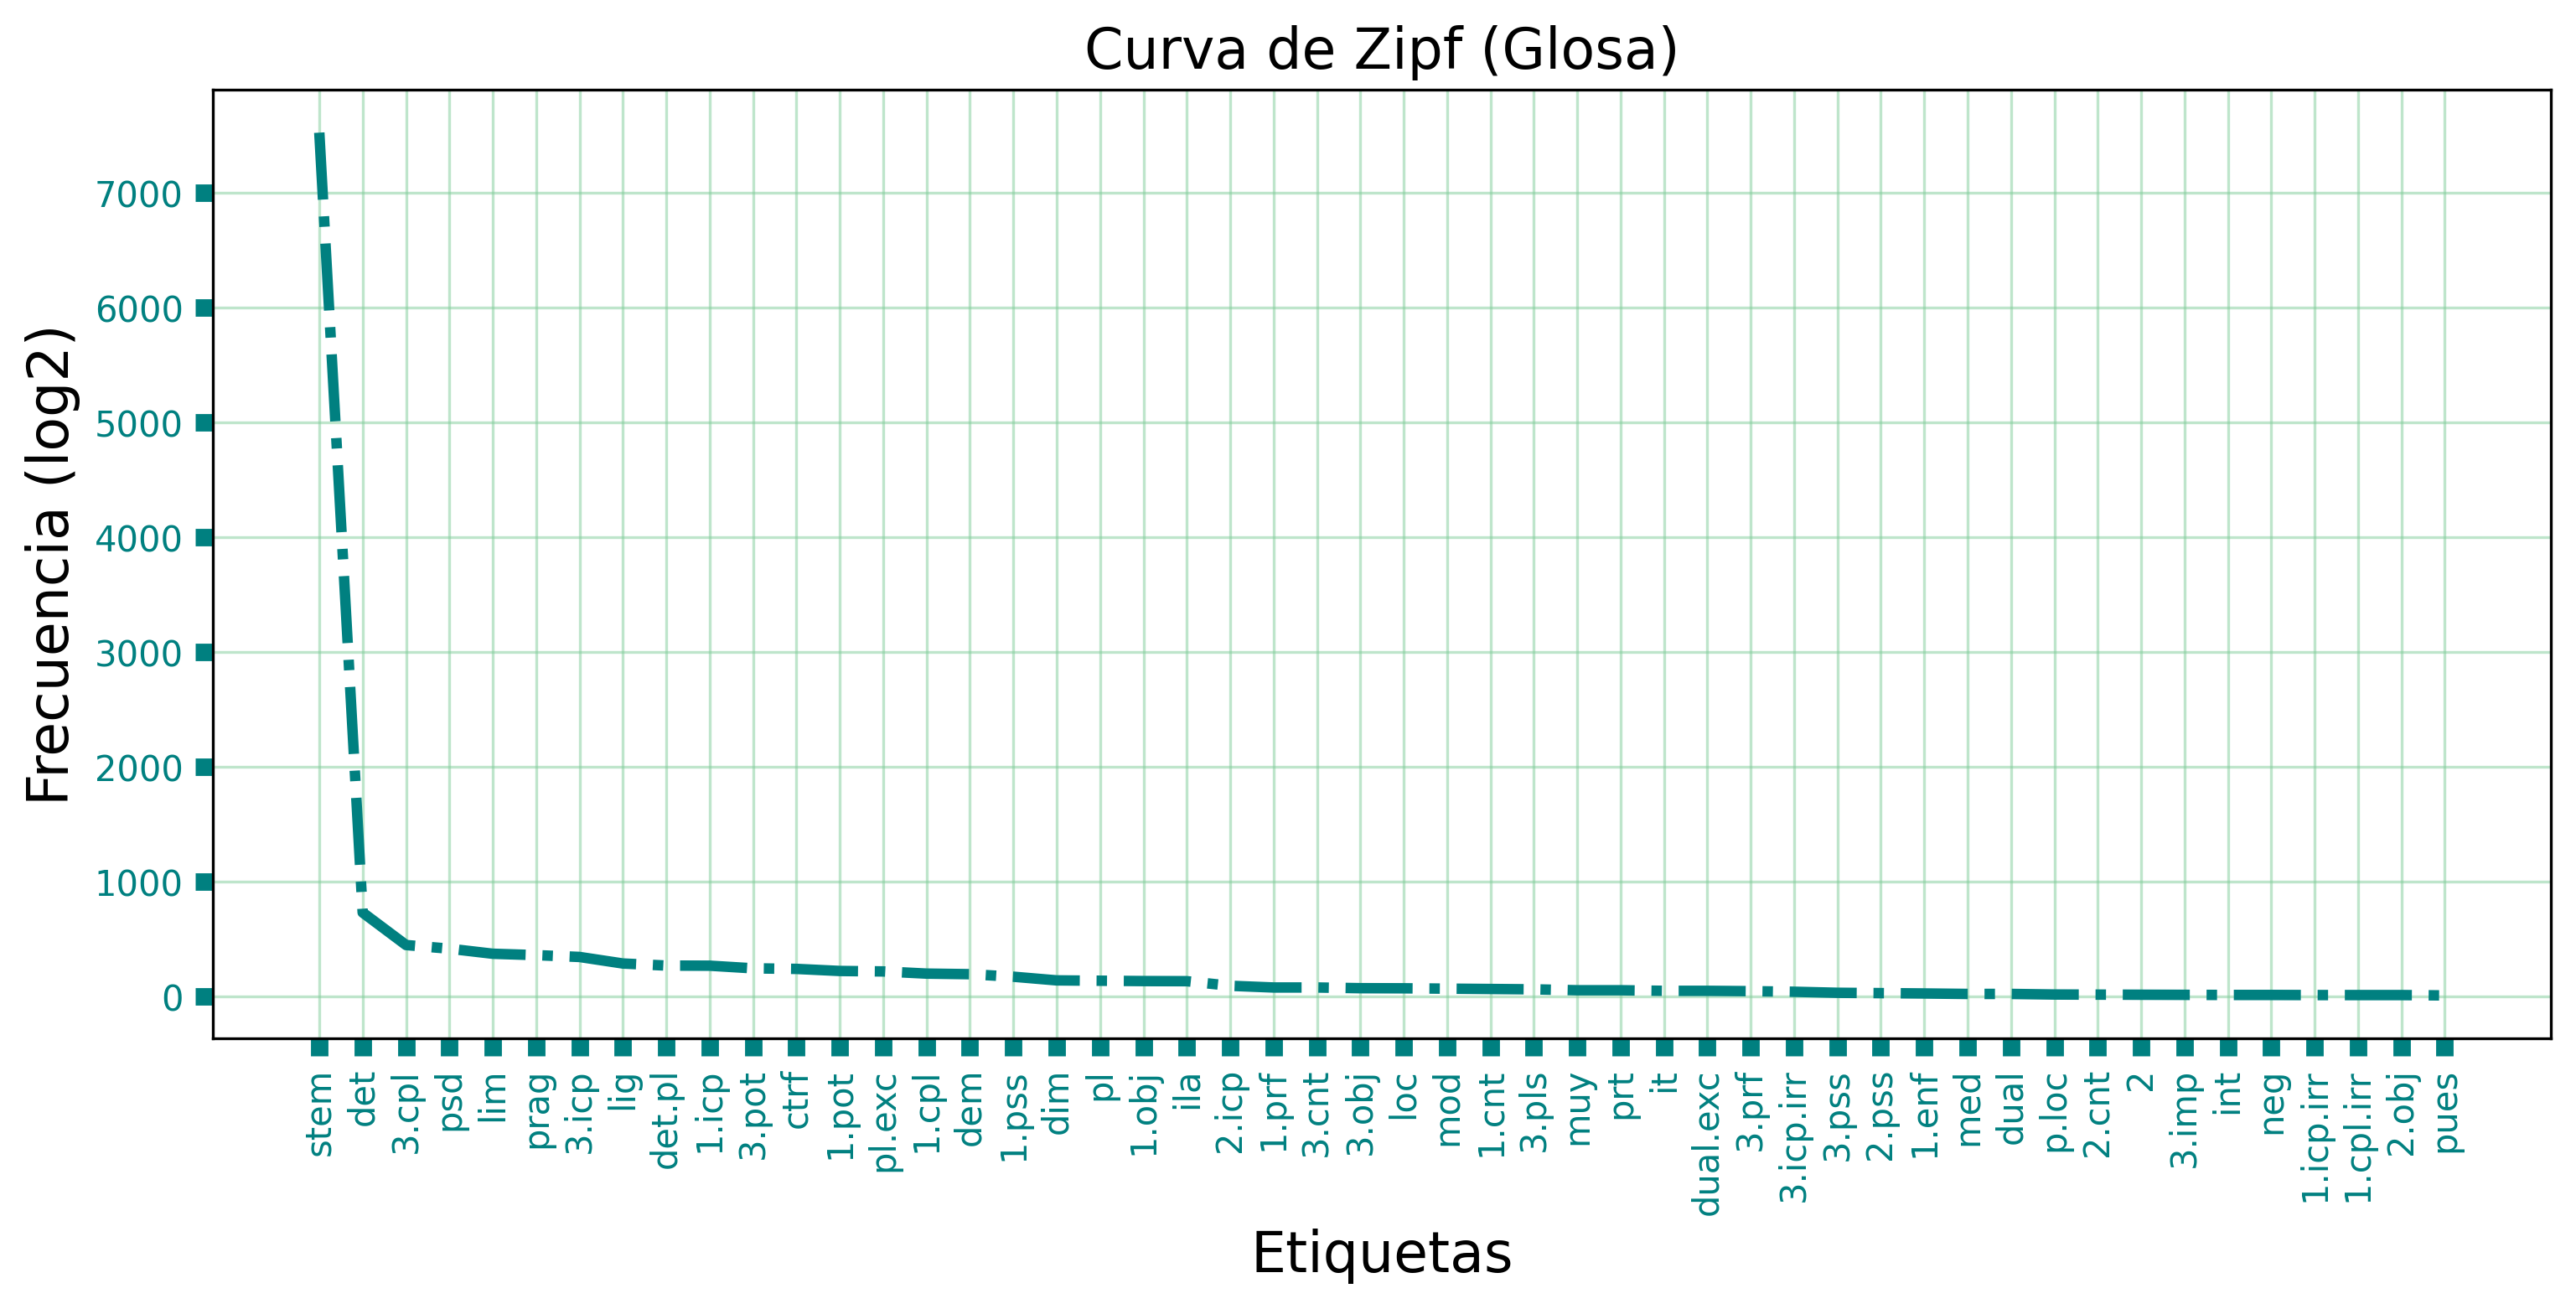
\includegraphics[width=\textwidth]{zipf_gloss}
	\caption{Distribución de glosa (primeras 50)}
	\label{fig:gloss_distrib}
\end{figure}

En las tablas \ref{table_pos_gloss_tokens} se muestran las cuentas de los diez tokens más comunes para las etiquetas \textit{POS} y para la glosa presentes en el corpus. Es destacable tanto la cantidad de oraciones etiquetadas, presentadas en la tabla \ref{table:corpus_length:1}, como la cantidad de tokens de la tabla \ref{table_pos_gloss_tokens} ya que representan un conjunto de textos ínfimo en comparación con los corpus utilizados en métodos de \textit{NLP} convencionales, donde, en general, su desempeño es altamente dependiente de grandes cantidades de textos.

Esta escasez en el corpus es consecuencia de que el idioma otomí es una lengua con bajos recursos digitales. Como menciona \citet{vasquesextraccion} estas lenguas son aquellas que tienen una cantidad limitada de recursos digitales a consecuencia de una baja densidad de hablantes, cuestiones relacionadas con la brecha digital o motivos de otra índole. Gran parte de los métodos tradicionales de \textit{NLP} tienen dificultades importantes para trabajar en entornos de bajos recursos.

\Diego{Cambiar redaccion, dado que hay bajos recursos el corpus es pequeño no al reves}

\begin{table}[h]
	\centering
	\begin{tabular}{|c | c|}\hline
		\textbf{Etiqueta \textit{POS}} & \textbf{Tokens} \\ \hline
		v & 2596 \\
		obl & 2447 \\
		det & 975 \\
		cnj & 837 \\
		dem & 543 \\
		unkwn & 419 \\
		n & 273 \\
		neg & 178 \\
		p.loc & 81 \\
		prt & 49 \\\hline
	\end{tabular}
	\quad
	\begin{tabular}{|c | c|}\hline                            
		\textbf{Glosa} & \textbf{Tokens} \\ \hline
		stem & 7527 \\
		det & 733 \\
		3.cpl & 450 \\
		psd & 418 \\
		lim & 374 \\
		prag & 362 \\
		3.icp & 346 \\
		lig & 289 \\
		det.pl & 271 \\
		1.icp & 270 \\\hline
	\end{tabular}
	\caption{Tokens de etiquetas (Primeras 10)}
	\label{table_pos_gloss_tokens}
\end{table}


Sin  embargo, el aprendizaje estructurado y, en concreto, los \textit{CRFs} prometen hacer frente a estas condiciones experimentales. Por ejemplo, los \textit{CRFs}, a diferencia de otros modelos gráficos, toman las virtudes de los modelos generativos y de los modelos condicionales evitando, a su vez, el problema del \textit{bias} que \citet{lafferty2001conditional} define como  ''el momento en el cual las transiciones que salen de un estado sólo compiten entre sí, y no con todas las demás transiciones'' 
% \Diego{Ya deben estar definidas que son las trancisiones en el marco teórico}.

\section{Arquitectura}

% Definir el método en función del marco teórico
% Diagrama de la arquitectura
% Feature functions
% Como se decidieron
% ¿Porque estas caracteristicas son reelevantes?
% Que es para nosotrxs una FF
% Experimentos quitando features functions
% Diagram de donde se encuentran estos elementos en la arquitectura
% Como se calculan lambdas y mu
% Variacion de hiperparámetros
% Descripcion de que variaciones se hicieron
% Hablar de L1 y L2 con ciertas combinaciones
% Mostrar el base line y compararlo
% Metodo de regularizacion y optimización
% Mencionar que se usará un base line
% ¿Cómo se hizo lo que se hizo?
% Preprocesamiento del corpus

Para esta tesis proponemos una arquitectura de aprendizaje estructurado débilmente supervisado utilizando el método gráfico \textit{Conditional Random Fields (CRF)} que permitirá la predicción de secuencias que describen las unidades morfológicas (glosa) dentro de una palabra en otomí. Ya que el resultado esperado es la generación de etiquetas \textit{BIO} que, en principio, dependen unas de otras, un método que construye el modelo de aprendizaje basandose en gráficas nos pareció adecuado.

Una vez obtenido el corpus, previamente glosado, realizamos una etapa de preprocesamiento del corpus, luego de esta etapa fueron creadas las \textit{feature functions}, que definimos como $X$. Tales funciones contienen información sobre la estructura de la lengua y permiten que lá máquina aprenda un modelo para etiquetar secuencias. Cabe señalar que $X$ son las entrada de los \textit{CRFs}.

Debido al enfoque de aprendizaje automático que estamos utilizando consideramos dos conjuntos; un conjunto de entrenamiento y otro de pruebas. Los conjuntos de entrenamiento y pruebas fueron fueron obtenidos del corpus que fue previamente glosados a mano por un experto lingüista.

La etapa de pruebas consistió en aplicar el modelo de aprendizaje al conjunto de evaluación. En ese sentido, aplicar el modelo se refiere a que con el modelo se generaron etiquetas \textit{BIO} para textos del conjunto de pruebas. Con las etiquetas generadas y en comparación con las etiquetas reales se obtuvieron, entre otras medidas de rendimiento, la precisión del modelo. Las secuencias de etiquetas o salidas generadas por el modelo, dadas las observaciones de $X$, fueron definidas como $Y$.

\Diego{Adapatar este parrafo para que tenga coherencia}

\begin{figure}
	\centering
	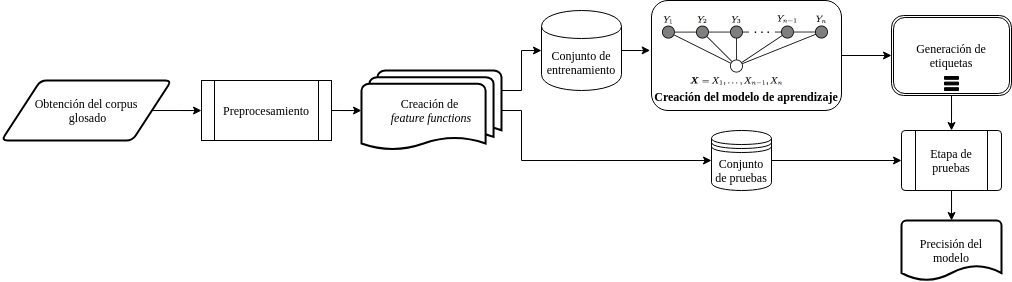
\includegraphics[width=\textwidth]{arquitectura}
	\caption{Arquitectura de aprendizaje}
	\label{fig:architecture}
\end{figure}

\Diego{ Diagrama}

\diego{¿Es pertinente esta información aquí?}
En general, para el glosado se realiza manualmente. Esta tarea requiere del expertiz del un lingüista y una cercana cooperación con hablantes nativos quienes reciben capacitación elemental en lingüística y software \citep{moeller2018automatic}. Estas condiciones convierten al glosado manual en una tarea altamente costosa en tiempo y recursos. El objetivo de esta arquitectura es realizar un correcto etiquetado automático de glosa para la lengua otomí, en particular la variante del otomí de Toluca, utilizando técnicas de aprendizaje estructurado débilmente supervisado. Con ello se pretende asistir a personas especializadas, como lingüistas, en el glosado manual.   

Parte de la definición de la estructura de la lengua se encuentra codificada en el conjunto de \textit{feature functions}. Estas funciones describen características de la lengua considerando, detalladamente, el contexto, la posición y etiquetas gramaticales que brindan información útil para la fase de entrenamiento.

Puntualmente, se utiliza un modelo del tipo \textbf{Markov CRF de primer orden con \textit{features} de estado y de transición}. Adicionalmente, fue utilizado el algoritmo de aprendizaje \textbf{Limited-memory Broyden-Fletcher-Goldfarb-Shanno (L-BFGS)}. El algoritmo busca maximizar el logaritmo de probabilidad. Para mejorar el rendimiento son utilizados y modificados un conjunto hiperparámetros.

Estos hiperparámetros son los coeficientes de regularización L1 y L2 necesarios para evitar posible \textit{overfitting}, el número máximo de iteraciones, el número máximo de memorias utilizadas para aproximar la matriz hessiana inversa, epsilon que determina la condición de convergencia, el número de iteraciones para probar el umbral de detención,  delta que define el umbral de detención de cada iteración, el método de búsqueda de línea usado por el algoritmo L-BFGS y el número máximo de intentos para el algoritmo de línea.
\Vic{Señalar los hiperparámetros que se utilizaron en L-BFGS}
El modelo y el algoritmo de aprendizaje fueron tratados a detalle en la sección \ref{sec:marco}.
\Diego{Descripción categorizada de los hiperparámetros}

La arquitectura propuesta abarca desde la obtención del corpus etiquetado, pasando por el preprocesamiento del mismo, llegando a la creación de las \textit{feature functions}, seguido de la separación de los datos en conjuntos de entrenamiento y pruebas, continuando con la fase de entrenamiento y construcción del modelo de aprendizaje, terminando en la etapa de pruebas compuesta por la generación de etiquetas y posterior comparación con la glosa real. Las subsecciones que componen esta arquitectura son \textbf{codificación y preprocesamiento}, \textbf{implementación de los CRFs} y \textbf{feature functions}. En el siguiente capítulo se abordaran las etapas de generación de glosa y pruebas.

La arquitectura de aprendizaje semi-supervisado para la generación de glosa para el otomí de Toluca se describe a continuación.

\subsection{Codificación y preprocesamiento}

Se obtuvo el corpus de un archivo de texto plano. Cada renglón de este archivo es una oración en otomí con glosa. Además, se tiene una etiqueta \textit{POS} por cada palabra. Las frases están estructuradas en forma de listas que contienen otras listas validas para el lenguaje \code{Python}.

La glosa esta presente por cada fragmento de las posibles palabras en otomí. Ejemplificando, la frase \textit{hi tótsogí} (`No lo he dejado') se representa en el corpus como se muestra en el ejemplo \ref{exmp:frase_glosada}.

Por último, la lengua otomí tiene una vasta variedad interna lo cual implica diferentes ortografías dependiendo de la región. Tomar en cuenta esta variación ortográfica es de suma importancia para el preprocesamiento. Como menciona \cite{elotl2019otomiprepro} todas las lenguas otomíes son tonales y distinguen entre vocales orales y vocales nasales, existen fonemas que pueden presentarse en unas variantes, mientras que en otras están ausentes. En general, las vocales orales incluyen a las mismas vocales que también se presentan en el español: a, e, i, o, u; pero su inventario de vocales orales no se limita a estas cinco.

\begin{table}[]
    \centering
    \begin{tabular}{|c c c c c c|}\hline
        IPA & \textipa{1} & \textipa{E} & \textipa{O} & \textipa{2} & \textipa{9} \\ \hline
        Ortografía práctica & $\b{u}$ & $\b{e}$ & $\b{a}$ & $\b{i}$ & $\b{o}$ \\
        Convención para este trabajo & $\mu$ & $\epsilon$ & $\alpha$ & $\iota$ & \\ \hline
    \end{tabular}
    \caption{Representación de cada vocal en IPA (alfabeto fonético internacional)}
    \label{tab:vocales_otomi}
\end{table}{}
\diego{Quitar los autores y dejar la ortografia práctica. Incluir la tabla de equivalencias}

Ya que el otomí presenta una amplia variedad de vocales, como se puede ver en la tabla, su representación digital puede suponer un reto por la falta de normalización o por la codificación. En nuestro caso, cuando se codificaban algunas vocales para ser representadas como cadenas eran separadas por el lenguaje de programación ocasionando un etiquetando de caracteres que por si solos no tiene sentido. Entonces, fue necesario modificar algunas de las vocales del otomí. Las equivalencias de tales modificaciones pueden observarse en la tabla \ref{tab:vocales_otomi}

\begin{exmp} \label{exmp:frase_glosada}
    \code{[[[`hi', `stem'], `neg'],
    [[`tó', `1.prf'],
    [`tsogí', `stem'], `v']]}
\end{exmp}
\Vic{En este caso, el ejemplo quedaría mejor más cerca de la referencia}
\Diego{Corrección del margen}

Entonces, la estructura de las listas, por renglón, tiene la estructura \code{[[[letras, glosa], [letras, glosa], ..., POS],...]}. Una vez que se obtuvo el corpus de entrenamiento se le aplicó preprocesamiento. El preprocesamiento consistió en asociar, a cada letra de cada palabra, dos elementos; la etiqueta \textit{POS} y una \textit{Bio Label} correspondiente a esa letra.

Retomando el ejemplo \ref{exmp:frase_glosada} y después de aplicar el preprocesamiento el resultado sería el que se muestra en el ejemplo \ref{exmp:frase_preproc}. Cabe señalar que las \textit{Bio Labels} asignadas dependieron de la posición de la letra como se explico en la sección \ref{sec:marco}.

\begin{exmp} \label{exmp:frase_preproc}
    \code{[[['h', 'neg', 'B-stem'], ['i', 'neg', 'I-stem']], [['t', 'v', 'B-1.prf'],
          ['ó', 'v', 'I-1.prf'],
          ['t', 'v', 'B-stem'],
          ['s', 'v', 'I-stem'],
          ['o', 'v', 'I-stem'],
          ['g', 'v', 'I-stem'],
          ['í', 'v', 'I-stem']]]}
\end{exmp}{}
\Diego{Correccion del margen}

Con las palabras etiquetadas a nivel de letra se obtuvo un conjunto de entrenamiento y un conjunto de pruebas. Por una parte, el conjunto de entrenamiento permitió la observación de ejemplos y la posterior generación de un modelo de aprendizaje. Por otro lado, con el conjunto de pruebas obtuvimos la precisión del modelos etiquetando frases no vistas. Es importante destacar que estos dos conjuntos estuvieron completamente separados ya que mezclar el conjunto de entrenamiento y de pruebas pudo habernos llevado a una precisión erronea y sesgada.

Previo al entrenamiento se construyeron las \textit{feature functions} con el conjunto de entrenamiento. En ese sentido, por cada letra etiquetada de las palabras en otomí se tuvo una \textit{feature function} y por cada \textit{feature function} se tiene una \textit{Bio Label} asociada. La construcción de estas funciones será descrita a profundidad en la subsección \ref{subsec:feature}.

% Entrenamiento

Los \textit{CRFs} recibieron como entrada las \textit{feature functions}, representadas por un vector $X$ y sus respectivas \textit{Bio Labels}, representadas por un vector $y$, asociadas con cada \textit{feature function} con concordancia uno a uno respetando la posición. 

% Feature functions
\subsection{Feature functions} \label{subsec:feature}

La extracción de estas características es importante porque capturar fenómenos lingüísticos necesarios para que la estructura de la lengua se pueda plasmar en el modelo de aprendizaje. Estas características están capturando, entres otras cosas, el contexto de la palabra y es importante para predecir la morfología. Para construir las \textit{feature functions} se necesita el corpus glosado y etiquetado a nivel de letra. Se extrajeron las siguientes características para cada letra en el corpus:

\Vic{Pasar a formato de description}
\begin{description} \label{feature_functions_descr}
    \item[Bias:] Esta característica captura la proporción de una etiqueta dada en el conjunto de entrenamiento. El modelo aprende los pesos asociados con las etiquetas como si las etiquetas se generaran independientemente de una distribución de probabilidad dada. Ayuda a tomar en cuenta que algunas etiquetas son poco usuales y otras muy usuales.
    
    \item[\textsf{letterLowercase}:] Toma la letra y la convierte a minúsculas. Es importante para la creación del modelo tener en cuenta la letra que se esta viendo en un momento determinado para las predicciones posteriores. 
    
    \item[\textsf{prevpostag} y \textsf{nxtpostag}:] Es conveniente y muy útil tomar en cuenta las etiquetas \textit{POS} ya que brindan información gramatical de la palabra que se observa en ese momento. Tal información se basa en la morfología y algunas veces en la sintaxis de la lengua.

    \textsf{prevpostag} toma la etiqueta POS previa (Si existe) y \textsf{nxtpostag} toma la etiqueta POS siguiente (Si existe)
    
    \item[\textsf{BOS}, \textsf{EOS}, \textsf{BOW} y \textsf{EOW}:] Indicar el inicio y fin de frase y palabras otorga la capacidad de ver que tipo de palabras se está viendo en ese momento. Por ejemplo, transiciones que propician estados iniciales y finales brindan información contextual.

    \textsf{BOS} indica el inicio de la frase, \textsf{EOS} indica el fin de la frase \textsf{BOW} indica el inicio de la palabra y \textsf{EOW} indica el final de la palabra.
    
    \item[\textsf{letterposition}:] Indica la posición de la letra en la palabra. Otorga más información sobre el contexto de la palabra en la frase que se observa en un determinado momento.
    
    \item[\textsf{prev<n>letters} y \textsf{nxt<n>letters}:] La recuperación de ventanas de contexto son convenientes para del otomí ya que se trata de una lengua aglutinante dónde, en general, las palabras son largas. En particular, la longitud promedio de las palabras en el corpus es de 4.89\footnote{Promedio de la distribución de palabras basada en  en tokens. Para una distribución por tipos se obtuvo 7.2}. Esta característica da la pauta para que la observación del contexto en un determinado momento sea relevante para la construcción del modelo.
    
    \textsf{prev<n>letters} toma las $n$ letras previas y \textsf{nxt<n>letters} toma las $n$ letras siguientes, si existen en ambos casos. La variable $n$ determina el nombre de la \textit{feature} que indica el tamaño de la ventana a partir de la letra que se esta viendo en ese momento y va desde el número uno, caso dónde no se incluye número en el nombre, hasta el número cuatro. Por ejemplo, \textsf{prev4letters} toma las cuatro letras previas y \textsf{nxtletter} toma la letra siguiente.
\Diego{Separar next y prev}
\Diego{utilizar prevkletter y describir que es k}
\end{description}
\Diego{Pasar al entorno de descripcion}


Las características mencionadas son información relevante para poder construir un modelo más preciso dadas las estructuras de la lengua. Dichas características pueden o no estar presentes dependiendo de la letra que se esté viendo en ese momento. Por ejemplo, si es la primer letra de una palabra la que se observa no estarán presentes las características \textsf{prevletter}, \textsf{prev2letters} o \textsf{EOW} por mencionar algunas. Características como \textsf{letterLowercase} o \textsf{bias} siempre estuvieron presentes.

La construcción de las \textit{feature functions} dependió del experimento en turno. Por ejemplo, en algunos casos fueron modificadas reduciéndolas ignorando las etiquetas que brindaban información gramatical o fueron construidas para solo observar la letra actual y la anterior simulando un \textit{Hidden Markov Model (HMM)} utilizando \textit{CRFs}.


% hiperparámetros
\subsection{Implementación de CRFs y entrenamiento}

El termino \textit{CRFs} se refiere a una familia de métodos de aprendizaje basados en gráficas. En concreto, para la generación de secuencias de etiquetas utilizamos \textit{linear-chain CRF}. Este método requiere de un algoritmo de optimización. Como ya mencionamos previamente utilizamos el \textit{L-BFGS}. Este algoritmo mejora los pesos de las funciones muy lentamente al comienzo de un proceso de entrenamiento, pero al final converge rápidamente en los pesos óptimos de las funciones.

El entrenamiento consistió en la búsqueda de un modelo que maximiza el logaritmo de verosimilitud con el método de aprendizaje \textit{L-BFGS}. Es necesario entonces definir los parámetros del algoritmo de maximización. Los hiperparámetros modificados fueron los de \textit{Elastic Net} con valores de regularización L1 + L2. También, fue configurado el número máximo de iteraciones para el algoritmo pero fue fijado en 50 para todos los modelos. El resto de hiperparámetros se dejaron con un valor predeterminado. En la tabla \ref{tab:hyper_default_values} se muestran los valores que no se modificaron para los hiperparámetros.

\begin{table}[]
    \centering
    \begin{tabular}{| c | c |}\hline
        \textbf{Hiperparámetro} & Valor \\\hline
        \textsf{max\_iterarions} & 50 \\
        \textsf{num\_memories} & 6 \\
        \textsf{epsilon} & \num{1e-5} \\
        \textsf{stop} & 10 \\
        \textsf{delta} & \num{1e-5} \\
        \textsf{linesearch} & ''MoreThuente'' \\
        \textsf{max\_linesearch} & 20 \\\hline
    \end{tabular}
    \caption{Valores de los hiperparámetros}
    \label{tab:hyper_default_values}
\end{table}
\Diego{Mencionar los hiperparámetros seteados por defecto}

Además de los hiperparámetros se configuraron diferentes entornos de experimentación dónde se construyeron \textit{feature functions} con mas o menos información. En la tabla \ref{tab:models-config} se listan las diferentes configuraciones implementadas en esta tesis.

% Modelos

\begin{table}[ht]
    \centering
    \begin{tabular}{| c | c | c | c | c |}\hline
        \textbf{Modelo} & \textbf{L1} & \textbf{L2} & \textbf{Tiempo} & \textbf{Precisión}\\ \hline
        \textsf{linearCRF\_l2\_zero} & 0.1 & 0 & 41.86 [m] & 0.9516\\
        \textsf{linearCRF\_featured} & 0.1 & \num{1e-3} & 42.91 [m] & 0.9509\\
        \textsf{linearCRF\_l1\_l2\_zero} & 0 & 0 & 39.46 [m] & 0.9499\\
        \textsf{POS\_Less} & 0.1 & \num{1e-3} & 37.91 [m] & 0.9499\\
        \textsf{linearCRF\_l1\_zero} & 0 & \num{1e-3} & 41.03 [m] & 0.9480\\
        \textsf{POS\_Less\_l1\_zero} & 0 & \num{1e-3} & 40.25 [m] & 0.9473\\
        \textsf{POS\_Less\_l1\_l2\_zero} & 0 & 0 & 36.67 [m] & 0.9452\\
        \textsf{HMMLike\_l2\_zero} & 0.1 & 0 & 43.71 [m] & 0.8818\\
        \textsf{HMMLike\_regularization} & 0.1 & \num{1e-3} & 42.98 [m] & 0.8791\\\rowcolor{Yellow}
        \textsf{baseline\_HMMLike\_zero} & 0 & 0 & 40.44 [m] & 0.8762\\
        \textsf{HMMLike\_l1\_zero} & 0 & \num{1e-3} & 43.90 [m] & 0.8745\\\hline
    \end{tabular}
    \caption{Modelos de aprendizaje}
    \label{tab:models-config}
\end{table}

\Diego{El mas alto, mas bajo, el POS y el baseline}
\Diego{Todo en una sola tabla}


% Testing
Terminada la fase de entrenamiento y construido el modelo de aprendizaje se puso a prueba con el conjunto destinado a este propósito y que fue previamente obtenido. Similar a la fase de entrenamiento las entradas fueron las \textit{feature functions} y la \textit{Bio Labels} asociada a cada \textit{feature function}. Utilizando el modelo de aprendizaje se etiquetó cada letra con base en la estructura de la lengua codificada en las \textit{feature functions}. Las etiquetas generadas fueron comparadas con las reales y con ello se obtuvo la exactitud del modelo. 

\subsubsection{Hardware utilizado}

En la fase de experimentación fue utilizado el paquete \textsf{python-crfsuite} que es un \textit{binding} de la implementación de \citet{CRFsuite} para CRFs para lenguaje de programación \textit{Python} en su versión \textit{3.7}. La fase de experimentación corrió en una maquina con un procesador \textsf{Intel i7-7700HQ @ 3.800GHz} con \textsf{16 GB} de memoria principal. En promedio una corrida de entrenamiento y evaluación \textit{K-folds} con \textit{k=10} tomó 52 minutos.


Recapitulando.... 
% TODO: Resumen al final (pasos de todo lo que se hizo) como puntos o un diagrama

\chapter{Resultados}
% Solo reportar

En este capítulo se examinará el método de evaluación utilizado para la construcción de los modelos de aprendizaje. Además, se detallará el desempeño de los modelos que fueron mencionados en el capítulo \ref{chap:metodology} y se profundizará en los resultados obtenidos en los diferentes entornos de experimentación. 

% Mostrar la comparación a profundidad del baseline con todos los experimentos
% Demostrar que lo que propusimos fue mejor
% Cualitativos y cuantitativos
% Hablar del Baseline y como mejoró con mas features
% explicar como ayudo la información de las Feature functions
% Definir como plantear la historia: 
    % De lo mas básico (baseline) y ver como lo mejoramos con las feature functions
    % El conocimiento lingüístico ayuda a mejorar

\section{Evaluación}

Propusimos diferentes entornos de experimentación dónde fueron modificadas las \textit{feature functions} y los parámetros de regularización \textit{Elastic Net} L1 + L2. En concreto, se presentaron tres entornos de evaluación; en el primero se redujeron las \textit{features} al mínimo, utilizando la información de la letra actual en la palabra y la letra anterior relativa a la letra actual, con lo que se simulaba un \textit{Hidden Markov Model (HMM)}; en el segundo, se modificaron las \textit{features} para ignorar las etiquetas \textit{POS}, y en el último, se utilizaron todas las \textit{features} disponibles, que se mencionaron en la sección \ref{feature_functions_descr}.

En ese sentido, para evaluar el desempeño de los modelos construidos, presentes en la tabla \ref{tab:models-config}, seleccionamos como base el entorno dónde se simula un \textit{HMM} que corresponde con el modelo \textsf{baseline\_HMMLike\_zero}. 

% Pasar a resultados
Para determinar la precisión utilizamos una técnicas típica de \textit{ML} llamada \textit{cross-validation K-folds} que consiste en tomar \textit{K} fragmentos aleatorios del conjunto de entrenamiento y utilizarlos como conjunto de pruebas para evaluar el modelo. Consideramos exitosa la predicción si se logra maximizar la correcta clasificación de las secuencias de salida. La determinación del corpus de evaluación se explica a continuación.

Para cada modelo, se sacaron $K$ fragmentos del conjunto de entrenamiento. Cada fragmento fue utilizado como conjunto de evaluación por lo que el entrenamiento-evaluación se realizó $K$ veces por modelo. Para todas las etapas de entrenamiento-evaluación utilizamos $K = 10$. Por cada modelo se obtuvieron $K$ precisiones, una por cada conjunto de entrenamiento-evaluación, por lo que fueron promediadas para tener una precisión general por modelo que es la que reportamos.

% Aquí se habla del K fold 

A continuación mencionamos los modelos resultantes de cada una de las tres etapas de experimentación propuestas en este trabajo.

En la tabla \ref{tab:models-full-featured} se muestran los modelos dónde se recuperaron todas las \textit{features} disponibles

\begin{table}[ht]
    \centering
    \begin{tabular}{| c | c | c | c |}\hline
    \textbf{Modelo} & \textbf{Precisión} & $L_1$ & $L_2$\\\hline
    \textsf{linearCRF\_l2\_zero} & 0.9516 & 0.1 & 0\\
    \textsf{linearCRF\_featured} & 0.9509 & 0.1 & 0.001\\
    \textsf{linearCRF\_l1\_l2\_zero} & 0.9499 & 0 & 0\\
    \textsf{linearCRF\_l1\_zero} & 0.948 & 0 & 0.001\\\hline
    \end{tabular}
    \caption{Modelos con todas las \textit{features} disponibles}
    \label{tab:models-full-featured}
\end{table}

En la tabla \ref{tab:models-pos-less} se encuentran los modelos que pertenecen al entorno de experimentación donde fueron ignoradas las etiquetas \textit{POS}

\begin{table}[ht]
    \centering
    \begin{tabular}{| c | c | c | c |}\hline
    \textbf{Modelo} & \textbf{Precisión} & $L_1$ & $L_2$\\\hline
    \textsf{POS\_Less} & 0.9499 & 0.1 & \num{1e-3}\\
    \textsf{POS\_Less\_l1\_zero} & 0.9473 & 0 & \num{1e-3}\\
    \textsf{POS\_Less\_l1\_l2\_zero} & 0.9452 & 0 & 0\\\hline
    \end{tabular}
    \caption{Modelos donde se ignoran las etiquetas \textit{POS}}
    \label{tab:models-pos-less}
\end{table}

En la tabla \ref{tab:models-hmmlike} se aprecian los modelos generados en el entorno de experimentación con las \textit{feature functions} reducidas al mínimo, simulando \textit{HMMs}.

\begin{table}[ht]
    \centering
    \begin{tabular}{| c | c | c | c |}\hline
    \textbf{Modelo} & \textbf{Precisión} & $L_1$ & $L_2$\\\hline
    \textsf{HMMLike\_l2\_zero} & 0.8818 & 0.1 & 0\\
    \textsf{HMMLike\_regularization} & 0.8791 & 0.1 & \num{1e-3}\\
    \textsf{baseline\_HMMLike\_zero} & 0.8762 & 0 & 0\\
    \textsf{HMMLike\_l1\_zero} & 0.8745 & 0 & \num{1e-3}\\\hline
    \end{tabular}
    \caption{Modelos que simulan \textit{HMMs}}
    \label{tab:models-hmmlike}
\end{table}

\section{Análisis de resultados}

Comparando los diferentes entornos de entrenamiento y generación de modelos, observamos que, dado el escaso tamaño del corpus de entrenamiento, al recuperar mayor información en la construcción de las \textit{feature functions} y con métodos basados en gráficas como los \textit{CRFs} se obtiene un desempeño mayor en comparación con los entornos dónde las \textit{feature functions} tenían información mínima simulando métodos tradicionales de generación de etiquetas como los \textit{HMMs}.

% Hablar de HMM
% cual salio peor
En principio, el entorno de experimentación dónde simulamos \textit{HMMs} fue el que tomamos como base para poder comparar el desempeños de los \textit{CRFs}. Es importante destacar es una simulación ya que fueron útilizados los \textit{CRFs} para la construcción de estos modelos. En la tabla \ref{tab:models-hmmlike} se pueden ver los modelos construidos. Por una parte,  el modelo con la precisión más baja se encuentra en este entorno de experimentación y es \textsf{HMMLike\_l1\_zero} con $87.45\%$. Por otra parte, el modelo propuesto como base supera al modelo \textsf{HMMLike\_l1\_zero} por apenas \num{1.7e-3} puntos de precisión. Notamos que solo variando los hiperparametros $L_1$ y $L_2$ para este entorno de experimentación se obtuvo una mejora de apenas \num{5.6e-3} puntos de precisión respecto al modelo base.

% Hablar de POSLess
Continuando con el segundo entorno de experimentación, dónde se construyó el \textit{linear Chain CRF} ignorando las etiquetas \textit{POS}, la precisión mejoró de forma considerable respecto a los modelos que simulaban \textit{HMMs}. Como se puede ver en la tabla \ref{tab:models-pos-less} todos los modelos de este entorno lograron al menos una precisión del $94\%$. Observamos una mejora poco significativa con la variación de los hiperparametros $L_1$ y $L_2$. En este entorno el modelo con mayor precisión fue \textsf{POS\_Less} con $94.99\%$. 

Por último, el entorno dónde se tomaron todas las \textit{features} disponibles, mencionadas en \ref{feature_functions_descr}, fue en el que se obtuvo el mejor desempeño. Los modelos generados en este entorno obtuvieron entre $94\%$ y $95\%$ de precisión. Una vez más, la variación de hiperparametros comprobó mejoras leves en los modelos. Destacamos además que la mejora con respecto al entorno de experimentación anterior es de apenas $1\%$ en los modelos con mejor desempeño. En la tabla \ref{tab:models-comparation} se muestra la comparación entre el modelo base y los modelos con mejor precisión en los otros entornos de experimentación.

\begin{table}[ht]
    \centering
    \begin{tabular}{| c | c |}\hline
        \textbf{Modelo} & \textbf{Precisión} \\\hline
        \textbf{\textsf{linearCRF\_l2\_zero}} & \textbf{0.9516}\\ 
        \textsf{POS\_Less} & 0.9499\\ 
        \textsf{baseline\_HMMLike\_zero} & 0.8762\\ \hline
    \end{tabular}
    \caption{Comparación de modelos de diferentes entornos con mejor precisión}
    \label{tab:models-comparation}
\end{table}  

% logramos pasar el base line?
% que features fueron determinantes?
% Cual salio mejor
Con base en la arquitectura propuesta observamos que el modelo  \textbf{\textsf{linearCRF\_l2\_zero}} obtuvo la mejor precisión y que supera el modelo base propuesto \textbf{\textsf{baseline\_HMMLike\_zero}} (Ver tabla \ref{tab:models-comparation}). Del análisis a través de los entornos de experimentación podemos concluir, por un lado, que con la variación de hiperparametros en las tres familias de modelos (\textsf{linearCRF}, \textsf{POSLess}, \textsf{HMMLike}) (Ver tablas \ref{tab:models-full-featured}, \ref{tab:models-pos-less}, \ref{tab:models-hmmlike}), se obtuvo una mejora en la precisión poco representativa; por otra parte, la precisión que muestran los modelos \textsf{POSLess} y \textsf{linearCRF} es muy similar. Entonces, parece ser que la configuración de los hiperparametros \textit{Elastic Net} y las etiquetas \textit{POS}, codificadas en las \textit{feature functions}, mejoran levemente el desempeño de los modelos. Además, podemos concluir que el resto de información de la lengua, codificada también en las \textit{features functions}, son las que determinan, en gran medida, el desempeños de los \textit{CRFs} para la correcta generación de \textit{BIO Labels} (glosa) para el idioma otomí.  

\Diego{Poner gráfica de la función de perdida y comentar}


\chapter{Conclusiones}

\bibliography{tesis}
	
\end{document}
